\documentclass{article}

% https://www.cl.cam.ac.uk/local/typography/phd/#margin
\usepackage[a4paper, left=30mm, right=20mm, top=20mm, bottom=20mm]{geometry}

% Required for inserting images
\usepackage{graphicx}

\usepackage[utf8]{inputenc}
\usepackage[T2A,T3,T1]{fontenc}

\usepackage[backref=true]{biblatex}
\usepackage{biblatex}
\addbibresource{ref.bib}



% https://latex.org/forum/viewtopic.php?t=20320
\DeclareSymbolFont{tipa}{T3}{cmr}{m}{n}
\DeclareMathAccent{\invbreve}{\mathalpha}{tipa}{16} 

% To avoid "Too many math alphabets used in version normal."
% https://tex.stackexchange.com/questions/3676/too-many-math-alphabets-error
% https://tug.org/pipermail/yandytex/2003-September/000368.html
\newcommand\hmmax{0}
\newcommand\bmmax{0}

\usepackage{amsmath, amsfonts, amssymb, bm}

\usepackage{bbm} % For indicator function as \mathbbm{1}



\usepackage{yfonts}
\usepackage{mathrsfs}
\usepackage{pifont}
\usepackage{ifsym}
\usepackage{bbm}

\DeclareMathAlphabet\mathbfcal{OMS}{cmsy}{b}{n}
\usepackage{MnSymbol}
\usepackage{xcolor}
\usepackage[colorlinks=true]{hyperref}
\usepackage{caption}
\usepackage{subcaption}
\usepackage{tabularx}
\usepackage{epigraph} 
\usepackage{algorithm}
\usepackage{todonotes}
%\usepackage{algpseudocode}

\definecolor{darkblue}{rgb}{0.0, 0.0, 0.55}
\definecolor{forestgreen}{rgb}{0.13, 0.55, 0.13}
\definecolor{darkteal}{rgb}{0.0, 0.24, 0.18}

\hypersetup{
  linkcolor=darkblue,
  urlcolor=darkteal,
  citecolor=forestgreen
}

\definecolor{w}{RGB}{231, 160, 76}
\definecolor{l}{RGB}{37, 84, 138}

\newcommand{\wbox}{\textcolor{w}{\blacksquare}}
\newcommand{\lbox}{\textcolor{l}{\blacksquare}}

\newcommand{\wb}{\square}
\newcommand{\bb}{\blacksquare}


%For diagrams
\usepackage{tikz-cd}
\usetikzlibrary{decorations.pathreplacing,fit,shapes.geometric}

% To solve the potential \Cross error in bbding
\usepackage{savesym} 



\usepackage{environ}

\usepackage{amsthm}
\usepackage{etoolbox} % Required for \AtBeginEnvironment and \AtEndEnvironment

\theoremstyle{definition}

\newtheorem{definition}{Definition}[section]
\AtBeginEnvironment{definition}{%
  \pushQED{\qed}\renewcommand{\qedsymbol}{$\diamondsuit$}%
}
\AtEndEnvironment{definition}{\popQED}

\newtheorem{theorem}{Theorem}[section]
\AtBeginEnvironment{theorem}{%
  \pushQED{\qed}\renewcommand{\qedsymbol}{$\spadesuit$}%
}
\AtEndEnvironment{theorem}{\popQED}

\newtheorem{lemma}{Lemma}[section]
\AtBeginEnvironment{lemma}{%
  \pushQED{\qed}\renewcommand{\qedsymbol}{\rotatebox[origin=c]{180}{$\spadesuit$}}%
}
\AtEndEnvironment{lemma}{\popQED}

\newtheorem{conjecture}{Conjecture}[section]
\AtBeginEnvironment{conjecture}{%
  \pushQED{\qed}\renewcommand{\qedsymbol}{$\clubsuit$}%
}
\AtEndEnvironment{conjecture}{\popQED}

% Define the 'remark' environment with specific ending
\newtheorem*{remark}{Remark}
\AtBeginEnvironment{remark}{%
  \pushQED{\qed}\renewcommand{\qedsymbol}{$\triangle$}%
}
\AtEndEnvironment{remark}{\popQED}

% Define the 'example' environment with specific ending
\newtheorem*{example}{Example}
\AtBeginEnvironment{example}{%
  \pushQED{\qed}\renewcommand{\qedsymbol}{$\blacktriangle$}%
}
\AtEndEnvironment{example}{\popQED}


\AtEndEnvironment{lemma}{\popQED}

\renewcommand\qedsymbol{\textbf{Q.E.D.} \  $\heartsuit$}



% Supp
\DeclareMathOperator\supp{supp}

% Rotated Clubsuit
\usepackage{rotating}

\newcommand{\rotatedclubsuit}{\mathbin{\text{\begin{sideways}\begin{sideways}$\clubsuit$\end{sideways}\end{sideways}}}}


\usepackage{booktabs}
\usepackage{multirow}


% Multiple bibliography:
% https://tex.stackexchange.com/questions/98660/two-bibliographies-one-for-main-text-and-one-for-appendix
% https://www.overleaf.com/learn/latex/Questions/Creating_multiple_bibliographies_in_the_same_document

% ** *** ***** ******* ***********

\title{Ellsberg paradox \\
%Equilibrium predictive inference for Uniform distribution \\
        \large A minimal toy model}
\author{József Konczer\footnote{\href{mailto:konczer.j@gmail.com}{konczer.j@gmail.com},
        \href{https://konczer.github.io/}{konczer.github.io}}
        }
\date{February 2026}


\begin{document}

\maketitle

%\begin{abstract} 
%\end{abstract}

\section{Introduction}

In this draft I will analyze the two-colored Ellsberg paradox \cite{paper:Ellsberg1961}\footnote{A similar urn dilemma was introduced in Keynes's \emph{Treatise on Probability} (p. 75) \cite{book:TreatiseOnProbability} to illustrate the ``weight of argument''.} and show that there is a decision rule and a sharing group setting in which ambiguity aversion is emergent.

The following description is borrowed from a paper from 2017 (with some modifications to match the text to the figure and the original paper of Ellsberg):

\begin{quote}

Consider two urns each containing 100 balls (see Figure~\ref{fig:Ellsberg}).
The balls are either black or red. It is known that the first urn contains
exactly 50 black and 50 red balls. For the second urn however, the
composition of the colors is unknown.

\strut

\begin{figure}[H]
    \centering
    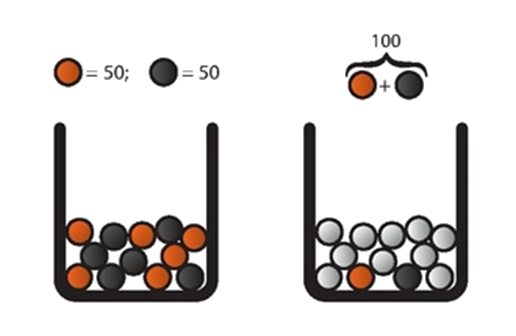
\includegraphics[width=0.4\textwidth]{img/Ellsberg-urn_alpha.png}
    \caption{The two Ellsberg urns: Urn 1 on the left contains well defined proportions of black and red balls, whereas for Urn 2 on the right the proportions are unknown.}
    \label{fig:Ellsberg}
\end{figure}

\strut

Subjects hold bets on the color of the balls to be drawn from the urns. A 
\emph{bet on black }``$b$'' yields $100$ Euro if the ball drawn from the urn
is black. Otherwise the payoff is zero. Similarly, \emph{betting on red }``$%
r$'', the subject earns $100$ Euro if a red ball is drawn and nothing
otherwise. Table~\ref{tab:Ellsberg} summarizes this choice problem.


\begin{table}[H]
\centering
\begin{tabular}{|l|c|c|c|c|}
\hline
& \multicolumn{2}{|c}{\emph{Urn 1}} & \multicolumn{2}{|c|}{\emph{Urn 2}} \\ 
\hline
& 50 & 50 & \multicolumn{2}{|c|}{100} \\ \hline
& \emph{Black} & \emph{Red} & \emph{Black} & \emph{Red} \\ \hline
$b$ (\emph{bet on black}) & $100$ & $0$ & $100$ & $0$ \\ \hline
$r$ (\emph{bet on red}) & $0$ & $100$ & $0$ & $100$ \\ \hline
\end{tabular}%
\caption{Payoff table (in Euros) for betting on \emph{black} or \emph{red} in the two urns.}
\label{tab:Ellsberg}
\end{table}


Holding a bet first on\emph{\ black} ($b$) and then on \emph{red }($r$),
subjects had to choose the urn on which they wanted to bet.

A large number of subjects, about 60 percent, choose to bet on the draw from
Urn 1 for both bets\footnote{%
The fact that subjects prefer to bet on the urn with the known proportion of
colors could be confirmed in many repetitions of the Ellsberg experiment. 
\cite{paper:AmbiguityReview} reviewed 39 experimental studies of the
Ellsberg experiments. They report a median number of 59 percent of ambiguity
averse subjects across all studies which they reviewed.}. These choices
clearly contradict the assumption that these subjects were maximizing subjective expected utility.

    
    \hfill --- Ellsberg's suggested thought experiment\footnote{The description has been borrowed from \cite{paper:EllsbergHilbert}, which is based on the original paper \cite{paper:Ellsberg1961}.}.
    \end{quote}

Although for a single agent a game-theoretic decision rule will not resolve the paradox \cite{essay:EssayOnUncertaintyKonczer2024} -- for any utility functions this decision rule suggest a strategy, selecting both the risky and the uncertain urn with equal 50\% chance -- for a resource sharing group of risk-averse players, ambiguity aversion can emerge in this decision-making framework.

The following set of requirements seems to generate ambiguity aversion:

\begin{itemize}
    \item Total or partial sharing of rewards among more than one player,
    \item Risk aversion of the players (i.e. concave utility functions associated with the potential shared gains),
    \item A game-theoretic approach to uncertainty (akin to minimax-regret decision rules) \cite{arxiv:ExtendedEquilibrium, essay:EssayOnUncertaintyKonczer2024, book:Savage},
    \item One of the following circumstances:
    \begin{itemize}
        \item Strongly correlated uncertain parameters for the sharing players, or
        \item A non-individualistic outlook of the sharing players (a form of ``team reasoning'' \cite{paper:TeamReasoning,book:TeamReasoning}).
    \end{itemize}
\end{itemize}

In the following sections I will demonstrate how ambiguity aversion can emerge in the simplest suitable constructions, while in the last section I show that the effect vanishes even for a pair of individualistic Agents whose uncertain parameter are not known to be strongly correlated (highlighting that simply the Extended Equilibrium solution \cite{arxiv:ExtendedEquilibrium} for risk-averse players is not enough to witness ambiguity aversion). 

\section{Two minimal setups}

\subsection{Shared uncertainty}

There are two players, Player 1 and Player 2, who act independently, but will share all their capital in the end.
Both of them can choose from two urns. The Risky-urn contains precisely one red and one black ball, while in the \underline{shared} Uncertain-urn, the players don't know how many red or black balls are present.
(To make the first example as simple as possible, let's imagine that the Uncertain-urn contains only one single -- red or black -- ball.)\footnote{The Risky-urn might or might not be shared. If the two players cannot coordinate or correlate their actions, then we get the same result in the case of shared and separate Risky-urns.} I.e. they know nothing, except that there is one ball in the Uncertain-urn which can be either red or black.

After choosing an urn (Risky ($R$) or Uncertain ($U$)), the players can pick a ball -- after potentially mixing the urn --, and they can win 100 units of money (e.g. pounds\footnote{GBP/EUR/USD.}) if the picked ball is red (\emph{bet on red}).

The two players need to make their urn choices independently, but in the end, they collect their prizes into a pot and divide the total amount equally.

So to reiterate the setup:
There are two players; each can independently choose from a Risky or a \underline{shared} Uncertain-urn, and in the end, the two players equally share their gains.

\subsection{Formal description}

Formally, both players have two actions regarding which urn they choose:

\begin{equation}
    \mathcal{A}_1 = \{ R, U \}, \quad
    \mathcal{A}_2 = \{ R, U \}
\end{equation}

While the Uncertain urn can contain a red ($r$) or a black ($b$) ball:

\begin{equation}
    \Theta = \{ r, b \}
\end{equation}

To track the consequences of possible state-action pairs, we can introduce the following notation:
$A_{\alpha} \oplus B_\beta \oplus \dots \oplus Z_\zeta$ will stand for a consequence, where the sharing players are gaining $A$ amount of monetary units with probability $\alpha$, $B$ amount of monetary units with probability $\beta$ etc. (Naturally for all possible consequences $\alpha + \beta + \dots + \zeta = 1$.)

By this notation, we can keep track of potential outcomes and their probabilities, and it will be easy to convert a consequence to numerical utilities:
$u(A_{\alpha} \oplus B_\beta \oplus \dots \oplus Z_\zeta)= \alpha \cdot u(A) + \beta \cdot u(B) + \dots + \zeta \cdot u(Z)$

Using this notation, we can list the (expected-) consequences of the Players' action and the potential parameter value:

When both players are choosing the Risky-urn, the consequences are independent of the parameter value, i.e. the balls in the Uncertain-urn.

\begin{equation}
    \mathcal{EC}(a_1=R,a_2=R;\theta=r) 
    =
    \mathcal{EC}(a_1=R,a_2=R;\theta=b) 
    =
    100_{1/4} \oplus 50_{1/2} \oplus 0_{1/4}
\end{equation}

When only one player is choosing the Uncertain-urn, the parameter value matters.

\begin{equation}
    \mathcal{EC}(a_1=R,a_2=U;\theta=r) 
    =
    \mathcal{EC}(a_1=U,a_2=R;\theta=r) 
    =
    100_{1/2} \oplus 50_{1/2}
\end{equation}

\begin{equation}
    \mathcal{EC}(a_1=R,a_2=U;\theta=b) 
    =
    \mathcal{EC}(a_1=U,a_2=R;\theta=b) 
    =
    50_{1/2} \oplus 0_{1/2}
\end{equation}

And when both players choose the Uncertain-urn, the consequences are certain for given parameter values.

\begin{equation}
    \mathcal{EC}(a_1=U,a_2=U;\theta=r) 
    =
    100
\end{equation}

\begin{equation}
    \mathcal{EC}(a_1=U,a_2=U;\theta=b) 
    =
    0
\end{equation}

In tabular form, the consequences look as follows:
% \usepackage{multirow}

\begin{table}[H]
\begin{center}
\begin{tabular}{|l l|c c|}
\hline
\multirow{1}{*}{$\mathcal{EC}$} & & $\theta=r$  & $\theta=b$\\
\hline
\multirow{2}{*}{$a_1=R$}
  & $a_2=R$ &
  $100_{1/4} \oplus 50_{1/2} \oplus 0_{1/4}$ &
  $100_{1/4} \oplus 50_{1/2} \oplus 0_{1/4}$\\
\cline{2-4}
  & $a_2=U$ &
  $100_{1/2} \oplus 50_{1/2}$ &
  $50_{1/2} \oplus 0_{1/2}$\\
\hline
\multirow{2}{*}{$a_1=U$}
  & $a_2=R$ &
  $100_{1/2} \oplus 50_{1/2}$ &
  $50_{1/2} \oplus 0_{1/2}$\\
\cline{2-4}
  & $a_2=U$ &
  $100$ &  $0$\\
\hline
\end{tabular}
    \caption{Consequence array for shared uncertainty.}
        \label{tab:ConsequenceSharedUncertainty}
\end{center}
\end{table}

\subsection{Shared identity}

We can relax the shared uncertainty assumption and still see ambiguity aversion if we assume players with ``shared identity'' i.e. non-individualistic players whose regret is not defined by the counterfactual question: ``What I could do better?'' but rather ``What \underline{we} could do better?''.

The description of the situation is almost the same as before, except that we don't assume that the two players are facing the same Uncertain-urns. The two players will need to choose separately from two Uncertain-urns; however, the contents of these urns can be correlated or uncorrelated.

\subsection{Formal description}

Formally, both players have the same two actions regarding which urn they choose (where both players can choose their own Uncertain-urn):

\begin{equation}
    \mathcal{A}_1 = \{ R, U \}, \quad
    \mathcal{A}_2 = \{ R, U \}
\end{equation}

While the Uncertain-urns can contain a red ($r$) or a black ($b$) ball:

\begin{equation}
    \Theta_1 = \{ r, b \}, \quad
    \Theta_2 = \{ r, b \}
\end{equation}

The complete set of possible uncertain parameters, $\Theta$, is the Cartesian product of the two parametersets:

\begin{equation}
    \Theta = \Theta_1 \times \Theta_2 = \{ (r,r), (r,b), (b,r), (b, b) \}
\end{equation}

We can list the (expected-) consequences of the Players' action and the potential parameter value:

When both players are choosing the Risky-urn, the consequences are independent of the parameter value, i.e. the balls in the Uncertain-urns.

\begin{equation}
    \mathcal{EC}(a_1=R,a_2=R;\theta) 
    =
    100_{1/4} \oplus 50_{1/2} \oplus 0_{1/4}
\end{equation}

When only one player is choosing the Uncertain-urn, the parameter value matters.

\begin{equation}
    \mathcal{EC}(a_1=R,a_2=U;\theta=(r,r)) 
    =
    100_{1/2} \oplus 50_{1/2}
\end{equation}

\begin{equation}
    \mathcal{EC}(a_1=R,a_2=U;\theta=(r,b)) 
    =
    50_{1/2} \oplus 0_{1/2}
\end{equation}

(While the content of the Uncertain-urn does not matter for the player who is choosing the Risky-urn, from these calculated consequences, all cases are determinable in which one player is choosing the Risky-urn, and the other the Uncertain-urn.)

When both players are choosing the Uncertain-urn, there are four possible cases:

\begin{equation}
    \mathcal{EC}(a_1=U,a_2=U;\theta=(r,r)) 
    =
    100
\end{equation}

\begin{equation}
    \mathcal{EC}(a_1=U,a_2=U;\theta=(r,b)) 
    =
    \mathcal{EC}(a_1=U,a_2=U;\theta=(b,r)) 
    =
    50
\end{equation}

\begin{equation}
    \mathcal{EC}(a_1=U,a_2=U;\theta=(b,b)) 
    =
    0
\end{equation}

The tabulated consequences look as follows:
% \usepackage{multirow}

\begin{table}[H]
\begin{center}
\begin{tabular}{|l l|c c c c|}
\hline
\multirow{1}{*}{$\mathcal{EC}$} & & $\theta=(r,r)$ & $\theta=(r,b)$ & $\theta=(b,r)$ & $\theta=(b,b)$\\
\hline
\multirow{2}{*}{$a_1=R$}
  & $a_2=R$ &
  $100_{1/4} \oplus 50_{1/2} \oplus 0_{1/4}$ &
  $100_{1/4} \oplus 50_{1/2} \oplus 0_{1/4}$ &
  $100_{1/4} \oplus 50_{1/2} \oplus 0_{1/4}$ &
  $100_{1/4} \oplus 50_{1/2} \oplus 0_{1/4}$\\
\cline{2-6}
  & $a_2=U$ &
  $100_{1/2} \oplus 50_{1/2}$ &
  $50_{1/2} \oplus 0_{1/2}$ &
  $100_{1/2} \oplus 50_{1/2}$ &
  $50_{1/2} \oplus 0_{1/2}$\\
\hline
\multirow{2}{*}{$a_1=U$}
  & $a_2=R$ &
  $100_{1/2} \oplus 50_{1/2}$ &
  $100_{1/2} \oplus 50_{1/2}$ &
  $50_{1/2} \oplus 0_{1/2}$ &
  $50_{1/2} \oplus 0_{1/2}$\\
\cline{2-6}
  & $a_2=U$ &
  $100$ & $50$ & $50$ & $0$\\
\hline
\end{tabular}
\caption{Consequence array for general uncertainty.}
    \label{tab:ConsequenceSharedUncertainty}
\end{center}
\end{table}


\subsection{Two tales}

\subsubsection{A tale of two brothers}

\begin{example}[The tale of two brothers]
There were two brothers -- Čech and Lech\footnote{See the legend of Forefather Čech on \href{https://en.wikipedia.org/wiki/Ancient_Bohemian_Legends\#Forefather_\%C4\%8Cech}{Wikipedia} or an extended version of the story in \cite{LegendsOfOldBohemia63}.} -- who were seeking new lands together.
After a long journey, they found fertile land, rich in bison and deer.
The two brothers took a look from a hill and settled separately with their people beside two large rivers: Čech in the West, becoming the forefather of the Czechs, and Lech not far to the East, establishing the nation of the Polish people.
It was late spring when they stopped and went their separate ways. Their greatest danger appeared to be the first winter because the weather and climate were unknown to them, the terrain was foreign, and seeds should already have been sown.
They made a solemn pact as insurance: before winter, whatever they gained, they would share equally.

Both brothers settled on an unfamiliar terrain, with unknown but similar weather and climate. Both had two main options: either start growing crops from the seeds they brought or go hunting the local wild beasts.
Agriculture could be lucrative, but yields were highly sensitive to weather. The harvest was either bountiful or miserable, depending on the rain and the length of the summer.
Hunting, if successful, also provided valuable gains, but it could be effectively done only at separate waterholes (both the Eastern and the Western locations had exactly two waterholes). However, there were migrating herds in the East and the West; they did not prefer either of the available drinking places over the other, and their migration patterns were unpredictable\footnote{Crucially, in the case of hunting, hunters can choose which waterhole to visit, thereby influencing their chances of success. If they choose between hunting grounds in an unbiased way, then their chances of success will be 50\%, independent of the herds’ migration patterns.}. Therefore, hunting was risky -- by randomly choosing a waterhole, the chances of success and failure were equal -- while agriculture was a deeply uncertain (i.e., ambiguous) choice.

Before winter, the brothers would come together and share their gains equally (either by selling all their bounty and sharing the money or by directly sharing their table).

Both a successful hunt and a good harvest provided nourishment for six months, and the brothers knew these prospects before deciding what to do.

The biting dilemma both brothers had to resolve was whether to choose risky hunting or ambiguous farming. The outcomes of both choices were unpredictable, but by hunting, they could reduce their combined risk -- because they could choose independently between the waterholes -- while the deeply uncertain weather was correlated, i.e., good and bad harvests occurred together over the land they might cultivate.
Therefore, hunting offered more opportunities for diversification, while agriculture could bring either fortune or a bad harvest across the region.

The brothers valued certain gains more than gambles; they would rather take a certain gain sufficient for three months than risk a gamble with a 50\% chance of resulting either in a gain sufficient for six months or in nothing\footnote{They would prefer the gamble over the fixed three-month gain only if the chances of winning a six-month reward would increase to 75\%.}.

{\it The decision:}
The brothers, once settled and having scouted their spots, had to choose between their possible actions. However, for such influential decisions, they frequently consulted their gods and the spirits, used magical devices or hired a shaman. In this case, each of them drew a five-pointed star, marked three points for hunting and the remaining two for farming and then let a sacred stone fall from above to the centre. Choosing the option to which the stone fell closest was considered the answer of the supernatural forces to this unresolvable dilemma.

It is left to us, the readers of this story, to judge if they acted wisely or foolishly.
How the story ended was not known, but what was certain was that they needed to face the consequences of their actions and live with their decisions.

\end{example}
\subsubsection{A tale of two twin brothers}

\begin{example}[The tale of two twin brothers]
There were two twin brothers -- Castor and Pollux, the Dioscuri\footnote{For cultural context, see Castor and Pollux on \href{https://en.wikipedia.org/wiki/Castor_and_Pollux}{Wikipedia} or Dioscuri on \href{https://www.britannica.com/topic/Dioscuri}{Britannica}. For more details, see \cite{book:Diascuri}.} -- who were not only alike but felt as one soul in two bodies.
Once, they separated for a year.
One made a journey to the West, while the other sailed to the East, each seeking fortune in distant foreign lands.
Before separating, they declared to each other what was natural to their hearts: whatever they gained, they would share equally upon their return.
Both ended up far apart in unfamiliar terrain, with unknown weather and climate. Both brothers had two main options: either start agriculture by growing crops and fruits or go hunting for boars or other wild beasts.
Agriculture could be lucrative, but yields were highly sensitive to weather. The harvest was either bountiful or miserable, depending on the rain.
Hunting, if successful, also provided valuable gains, but it could be effectively done only once a year at separate waterholes (both the Eastern and the Western locations had exactly two waterholes). However, the pack of thirsty animals did not prefer either drinking place over the other, and the pattern it followed was unpredictable. Therefore, hunting was risky -- by randomly choosing a waterhole, the chances of success and failure were equal -- while agriculture was a deeply uncertain (i.e., ambiguous) choice.

After their ventures, the brothers planned to return home and share their gains equally (either by selling all their bounty on Greek markets and sharing the money or by directly sharing their table).

Both a successful hunt and a good harvest provided resources for six months, and the brothers knew these prospects before deciding whether to start farming or hunting.

The biting dilemma both brothers had to resolve was whether to choose risky hunting or ambiguous farming. The outcomes of both choices were unpredictable, but by hunting, they could reduce their combined risk -- because they could choose independently between the waterholes -- while their agricultural outcomes might be correlated, i.e., good and bad harvests could occur together even over long distances.
Therefore, hunting offered more opportunities for diversification, while agriculture could bring either fortune or a bad harvest across the region.

The brothers valued certain gains more than gambles; they would rather take a certain gain sufficient for three months than risk a gamble with a 50\% chance of resulting either in a gain sufficient for six months or in nothing\footnote{They would prefer the gamble over the fixed three-month gain only if the chances of winning a six-month reward would increase to 75\%.}.

{\it The decision:}
Once they arrived at their destinations, the twin brothers had to choose between their possible actions. However, for such influential decisions, they frequently consulted their gods and oracles or used devices.

As heroes from the Greek lands, they were familiar with concepts from geometry. They drew a square and cut a red ribbon equal in length to the square's diagonal and a white ribbon equal in length to one of the square's sides.
They curled the ribbons on a spinning top, forming a full circle with a red and a white arc, with both ribbons at an equal distance from the spinning axis.

They spun the top, and when it stopped at the red ribbon, they went hunting, while the white region meant sowing wheat.

However, they bemoaned that they had not discussed such possibilities in advance when they were still together at their father's palace. If they had known what choices awaited them, they could have used a different correlated strategy. Using three sacred coins, they could have prearranged their collective action in the following way:
If the first coin landed on Heads, they would both go hunting. If the first coin landed on Tails and the second fell on Heads, both would go farming. Finally, if the first two coins landed on Tails, then, if the third one landed on Heads, Castor would hunt and Pollux would farm, while Pollux would hunt and Castor would farm if the final coin landed on Tails.

It is left to us, the readers of this story, to judge if they acted wisely or foolishly.
How the story ended was not known, but what was certain was that even the divine twins had to face the consequences of their actions and live with their decisions.

\end{example}

\section{Assumptions}

After the description of the decision problems, in this section, I aim to make further assumptions transparent and explicit.

\subsection{Associated utilities}

I will assume that the two players can associate \emph{utilities} with the possible shared gains.
Further, I assume that the two players have the same utility functions.
In the dilemmas, essentially three different final monetary outcomes can occur, to which we will associate the following numerical utilities:

\begin{equation}
u(0) = 0, \quad u(100) = 1, \quad u(50)=u_h \ge 1/2
\end{equation}

(For the utility of the half-price, $u(50)=u_h \ge (u(0)+u(100))/2 = 1/2$ is the formalisation of the players’ risk aversion.)

To evaluate the expected utility of a specific consequence, we will use the following formula:

\begin{equation}
u(a_{p_a} \oplus b_{p_b} \oplus c_{p_c})
=
p_a u(a) + p_b u(b) + p_c u(c)
\end{equation}

As a concrete example:

\begin{equation}
u(100_{1/4} \oplus 50_{1/2} \oplus 0_{1/4})
=
\frac{1}{4} u(100)+ \frac{1}{2} u(50) + \frac{1}{4} u(0)
=
\frac{1}{4} + \frac{1}{2}u_h
\end{equation}

Using these conventions, we can determine the expected utility matrix for both shared and general uncertainty scenarios:

\begin{table}[H]
\begin{center}
\renewcommand{\arraystretch}{1.3} % <- try 1.2–1.6
\begin{tabular}{|l l|c c|}
\hline
\multirow{1}{*}{$\mathcal{E}U_i$} & & $\theta=r$  & $\theta=b$\\
\hline
\multirow{2}{*}{$a_1=R$}
  & $a_2=R$ &
  $\frac{1}{4} +  \frac{1}{2} u_h$ &
  $\frac{1}{4} +  \frac{1}{2} u_h$\\
\cline{2-4}
  & $a_2=U$ &
  $\frac{1}{2} + \frac{1}{2} u_h$ &
  $\frac{1}{2} u_h$\\
\hline
\multirow{2}{*}{$a_1=U$}
  & $a_2=R$ &
  $\frac{1}{2} + \frac{1}{2} u_h$ &
  $\frac{1}{2} u_h$\\
\cline{2-4}
  & $a_2=U$ &
  $1$ &  $0$\\
\hline
\end{tabular}
\caption{Utility array for shared uncertainty.}
    \label{tab:UtilitySharedUncertainty}
\end{center}
\end{table}



\begin{table}[H]
\begin{center}
\renewcommand{\arraystretch}{1.3} % <- try 1.2–1.6
\begin{tabular}{|l l|c c c c|}
\hline
\multirow{1}{*}{$\mathcal{E}U_i$} & & $\theta=(r,r)$ & $\theta=(r,b)$ & $\theta=(b,r)$ & $\theta=(b,b)$\\
\hline
\multirow{2}{*}{$a_1=R$}
  & $a_2=R$ &
  $\frac{1}{4} +  \frac{1}{2} u_h$ & 
  $\frac{1}{4} +  \frac{1}{2} u_h$ & 
  $\frac{1}{4} +  \frac{1}{2} u_h$ & 
  $\frac{1}{4} +  \frac{1}{2} u_h$\\
\cline{2-6}
  & $a_2=U$ &
  $\frac{1}{2} + \frac{1}{2} u_h$ & 
  $\frac{1}{2} u_h$ & 
  $\frac{1}{2} + \frac{1}{2} u_h$ & 
  $\frac{1}{2} u_h$\\
\hline
\multirow{2}{*}{$a_1=U$}
  & $a_2=R$ &
  $\frac{1}{2} + \frac{1}{2} u_h$ & 
  $\frac{1}{2} + \frac{1}{2} u_h$ & 
  $\frac{1}{2} u_h$ & 
  $\frac{1}{2} u_h$\\
\cline{2-6}
  & $a_2=U$ &
  $1$ & 
  $u_h$ & 
  $u_h$ & 
  $0$\\
\hline
\end{tabular}
\caption{Utility array for general uncertainty.}
    \label{tab:UtilitySharedIdentity}
\end{center}
\end{table}


\subsection{The generalized minimax regret criteria}

In case of the shared uncertainty scenario -- of sharing but individualistic players -- we can use a generalized version of the minimax regret criteria applied to the deeply uncertain parameter.
I will use the concept of Extended Equilibrium, introduced in \emph{Non-Cooperative Games with Uncertainty} \cite{arxiv:ExtendedEquilibrium}.

If we assume that Player 2 is applying the following mixed strategy:

\begin{equation}
    \sigma_2(R) = P_2, \quad \sigma_2(U) = \bar{P}_2 = 1-P_2
\end{equation}

The expected effective utility matrix for Player 1 looks the following (see ``expected or effective utility matrices for each player'' defined in eq. (15) in \cite{arxiv:ExtendedEquilibrium}):

\begin{table}[H]
    \label{tab:EffectiveUtilitySharedIdentity}
\begin{center}
\renewcommand{\arraystretch}{1.3} % <- try 1.2–1.6
\begin{tabular}{| l|c c|}
\hline
\multirow{1}{*}{$E\mathcal{E}U_1$} & $\theta=r$  & $\theta=b$\\
\hline
  $a_1=R$ &
  $P_2(\frac{1}{4} +  \frac{1}{2} u_h) + \bar{P}_2 (\frac{1}{2} + \frac{1}{2} u_h)$ &
  $P_2(\frac{1}{4} +  \frac{1}{2} u_h) + \bar{P}_2 (\frac{1}{2} u_h)$\\
\cline{1-3}
  $a_1=U$ &
  $P_2(\frac{1}{2} + \frac{1}{2} u_h)+\bar{P}_2(1)$ &
  $P_2(\frac{1}{2} u_h) + \bar{P}_2 (0)$\\
\hline
\end{tabular}
\caption{Effective utility matrix for shared uncertainty.}
\end{center}
\end{table}

From which we can derive the following expected effective regret matrix for Player 1 (see ``effective regret matrix'' defined in eq. (17) in \cite{arxiv:ExtendedEquilibrium}):

\begin{table}[H]
\begin{center}
\renewcommand{\arraystretch}{1.3} % <- try 1.2–1.6
\begin{tabular}{| l|c c|}
\hline
\multirow{1}{*}{$E\mathcal{E}R_1$} & $\theta=r$  & $\theta=b$\\
\hline
  $a_1=R$ &
  $\frac{1}{4} P_2 + \frac{1}{2}(1-u_h) \bar{P}_2$ & 
  $0$\\
\cline{1-3}
  $a_1=U$ &
  $0$ & 
  $\frac{1}{4} P_2 + \frac{1}{2} u_h \bar{P}_2$\\
\hline
\end{tabular}
\caption{Effective regret matrix for shared uncertainty.}
    \label{tab:EffectiveRegretSharedUncertainty}
\end{center}
\end{table}

\subsection{Assumptions in case of shared identity}

As we mentioned, the core assumption in case of the players with shared identity, is that they consider regret not as individuals, asking: ``What I could do better?'' but as a team: ``What we could do better?''.

Technically, this means that players with shared identity will not derive effective regret matrices and assume that the other player's strategy was a kind of external random factor, but the maximum utility will be identified as the best action profile they could have been done as a team at a given parameter value.

This approach results the following regret array for both players:

\begin{table}[H]
    \label{tab:EffectiveRegretSharedIdentity}
\begin{center}
\renewcommand{\arraystretch}{1.3} % <- try 1.2–1.6
\begin{tabular}{|l l|c c c c|}
\hline
\multirow{1}{*}{$\mathcal{E}R_i$} & & $\theta=(r,r)$ & $\theta=(r,b)$ & $\theta=(b,r)$ & $\theta=(b,b)$\\
\hline
\multirow{2}{*}{$a_1=R$}
  & $a_2=R$ &
  $\frac{3}{4} -  \frac{1}{2} u_h$ & 
  $\frac{1}{4}$ & 
  $\frac{1}{4}$ & 
  $0$\\
\cline{2-6}
  & $a_2=U$ &
  $\frac{1}{2} - \frac{1}{2} u_h$ & 
  $\frac{1}{2}$ & 
  $0$ & 
  $\frac{1}{4}$\\
\hline
\multirow{2}{*}{$a_1=U$}
  & $a_2=R$ &
  $\frac{1}{2} - \frac{1}{2} u_h$ & 
  $0$ & 
  $\frac{1}{2}$ & 
  $\frac{1}{4}$\\
\cline{2-6}
  & $a_2=U$ &
  $0$ & 
  $\frac{1}{2} - \frac{1}{2} u_h$ & 
  $\frac{1}{2} - \frac{1}{2} u_h$ & 
  $\frac{1}{4} + \frac{1}{2} u_h$\\
\hline
\end{tabular}
\caption{Regret array for shared identity.}
\end{center}
\end{table}


\section{Game-theoretic equilibrium}

The core idea in the game-theoretic approach to uncertainty is that players are developing strategies against an imagined adversarial ``trickster’’ whose utility matrix is the decision-making player's regret.

\subsection{Individualistic players with shared uncertainty}

To make the equilibrium calculations simpler, we can utilise a simple lemma from game theory: if we change a single player's utility matrix by adding terms which are independent of her actions, then this will not affect her equilibrium strategies. (This can be simply confirmed by recalling the defining set of inequalities for a Nash equilibrium.)

From this simple observation follows that we get the same equilibrium strategies if we assume that the decision-making player is maximising her utility or her effective regret.
Therefore, finding equilibrium strategies can be redefined as solving zero-sum games, defined by the (negative of the) effective regret matrix.

It is straightforward to check that the one unique mixed equilibrium for a zero-sum game defined by the following regret matrix:

\begin{equation}
    \underline{\underline{R}}
    =
    \begin{bmatrix}
    r_1 & 0 \\
    0 & r_2 
    \end{bmatrix}
\end{equation}

Is:

\begin{equation}
    \sigma^* = \left ( \frac{r_2}{r_1+r_2}, \frac{r_1}{r_1+r_2} \right )
    , \quad
    \pi^* = \left ( \frac{r_2}{r_1+r_2}, \frac{r_1}{r_1+r_2} \right )
\end{equation}

Where $\sigma^*$ is the eqilibrium strategy for the ``row player'' (choosing between rows) while $\pi^*$  is the eqilibrium strategy for the ``column player'' (choosing between the columns).

Applying this equilibrium formula, the expected effective regret matrix in Table~\ref{tab:EffectiveRegretSharedUncertainty}, we get the following expression:

\begin{equation}
    P_1^*(P_2) = \frac{\frac{1}{4} P_2 + \frac{1}{2} u_h \bar{P}_2}{\frac{1}{4} P_2 + \frac{1}{2}(1-u_h) \bar{P}_2 +\frac{1}{4} P_2 + \frac{1}{2} u_h \bar{P}_2}
    =
     \frac{\frac{1}{4} P_2 + \frac{1}{2} u_h \bar{P}_2}{\frac{1}{2} }
     =
     \frac{1}{2} P_2 + u_h \bar{P}_2
\end{equation}

Either by referring to symmetry or applying the more involved requirement $P^*_1(P^*_2(P_1))=P_1$ we arrive to the following formula describing the probability of choosing the Risky-urn for both players in the Extended Equilibrium:

\begin{equation}
    \boxed{
    P^*_1=P^*_2=P^*=\frac{u_h}{1/2+u_h}
    }
\end{equation}

In particular if $u_h=3/4$, then $P^* = 3/5 = 60\%$, showing a preference for the Risky-urn over the Uncertain-urn.

\subsubsection{Check of calculation with concrete numbers}

If we assume that $u_h=3/4$ and $P^*_1=P^*_2=P^*=3/5$

\begin{equation}
    \underline{\underline{E\mathcal{E}U_1}}
    =
    \begin{bmatrix}
    3/5 (\frac{1}{4}+\frac{1}{2} \cdot \frac{3}{4}) + 2/5 (\frac{1}{2}+\frac{1}{2} \cdot \frac{3}{4})  & 3/5 (\frac{1}{4}+\frac{1}{2} \cdot \frac{3}{4}) + 2/5 (\frac{1}{2} \cdot \frac{3}{4}) \\
    3/5 (\frac{1}{2}+\frac{1}{2} \cdot \frac{3}{4}) + 2/5 (1) & 3/5 (\frac{1}{2} \cdot \frac{3}{4}) + 2/5 (0) 
    \end{bmatrix}
\end{equation}

\begin{equation}
    \underline{\underline{E\mathcal{E}U_1}}
    =
    \begin{bmatrix}
    \frac{15}{40} + \frac{14}{40}  & \frac{15}{40} + \frac{6}{40} \\
    \frac{21}{40} + \frac{16}{40} & \frac{9}{40} + 0
    \end{bmatrix}
    =
    \begin{bmatrix}
    29/40 & 21/40  \\
    37/40 & 9/40
    \end{bmatrix}
\end{equation} 

\begin{equation}
    \underline{\underline{E\mathcal{E}R_1}}
    =
    \begin{bmatrix}
    8/40 & 0  \\
    0 & 12/40
    \end{bmatrix}
\end{equation} 

And the equilibrium solution of the game $\left\langle \underline{\underline{E\mathcal{E}U_1}}, \underline{\underline{E\mathcal{E}R_1}} \right\rangle$ is indeed:

\begin{equation}
    \sigma^* = (3/5, 2/5), \quad
    \pi^* = (3/5, 2/5)
\end{equation}

And the expected utility and regret are:

\begin{equation}
    EE\mathcal{E}U_1=129/200 = 0.645, \quad
    EE\mathcal{E}R_1 = 3/25 = 0.12
\end{equation}

The results can be checked manually or by available Nash equilibrium solvers (\href{https://cgi.csc.liv.ac.uk/~rahul/bimatrix_solver/}{Online Bimatrix solver} is a free online page created by Rahul Savani, in Python \href{https://nashpy.readthedocs.io/en/stable/}{Nashpy} is available, while in Wolfram Mathematica \href{https://reference.wolfram.com/language/ref/FindMatrixGameStrategies.html}{\tt FindMatrixGameStrategies} can be used to find Nash equilibria.)

\subsection{Correlated equilibrium for players with shared identity}

If the two capital-sharing players with shared identity can correlate their actions, then they can act together as a team. The team's extended action set is $\mathcal{A}=\mathcal{A}_1 \times \mathcal{A}_2$. (While the deeply uncertain parameter set is $\Theta = \Theta_1 \times \Theta_2$.)

The utility matrix for this extended game is:

\begin{equation}
    \underline{\underline{\mathcal{E}U}}
    =
    \begin{bmatrix}
    \frac{1}{4} +  \frac{1}{2} u_h & 
    \frac{1}{4} +  \frac{1}{2} u_h & 
    \frac{1}{4} +  \frac{1}{2} u_h & 
    \frac{1}{4} +  \frac{1}{2} u_h\\
    \frac{1}{2} + \frac{1}{2} u_h & 
    \frac{1}{2} u_h & 
    \frac{1}{2} + \frac{1}{2} u_h & 
    \frac{1}{2} u_h\\
    \frac{1}{2} + \frac{1}{2} u_h & 
    \frac{1}{2} + \frac{1}{2} u_h & 
    \frac{1}{2} u_h & 
    \frac{1}{2} u_h\\
    1 & 
    u_h & 
    u_h & 
    0\\
    \end{bmatrix}
\end{equation}

And the derived regret matrix looks as follows:

\begin{equation}
    \underline{\underline{\mathcal{E}R}}
    =
    \begin{bmatrix}
    \frac{3}{4} -  \frac{1}{2} u_h & 
    \frac{1}{4} & 
    \frac{1}{4} & 
    0\\
    \frac{1}{2} - \frac{1}{2} u_h & 
    \frac{1}{2} & 
    0 & 
    \frac{1}{4}\\
    \frac{1}{2} - \frac{1}{2} u_h & 
    0 & 
    \frac{1}{2} & 
    \frac{1}{4}\\
    0 & 
    \frac{1}{2} - \frac{1}{2} u_h & 
    \frac{1}{2} - \frac{1}{2} u_h & 
    \frac{1}{4} + \frac{1}{2} u_h\\
    \end{bmatrix}
\end{equation}

By applying a game-theoretic decision-making framework \cite{essay:EssayOnUncertaintyKonczer2024, arxiv:ExtendedEquilibrium}, i.e. minimax regret criteria for this extended team game against the deeply uncertain factors, we can find the following correlated equilibrium:

\begin{equation}
    \boxed{\sigma^*= \left (u_h-\frac{1}{4},\frac{1-u_h}{2},\frac{1-u_h}{2},\frac{1}{4} \right)}, \quad
    \pi^*= \left ( \frac{1}{4}, \frac{1}{4}, \frac{1}{4},\frac{1}{4} \right)
\end{equation}

(The result can be checked directly by calculating the expected utilities for all action -- given the equilibrium prior $\pi^*$ -- and the expected regrets for all parameter values -- given the equilibrium strategy $\sigma^*$.)

In particular, for $u_h=3/4$ we get:

\begin{equation}
    \sigma^*= \left (\frac{1}{2},\frac{1}{8},\frac{1}{8},\frac{1}{4} \right)
\end{equation}

\subsection{Independent actions with shared identity}

If the two capital-sharing players with shared identity are unable to act in a correlated way, then they can still try to find the best pair of independent strategies that would minimise their expected worst-case regret. This definition of a solution concept appears to be closer to the Regret Minimizing Equilibria (introduced by Nathanael Hyafil, Craig Boutilier) \cite{arxiv:RegretMinimizingEquilibria} (because here we are not explicitly searching for an equilibrium prior $\pi^*$).

Formally they can search for a pair of probabilities $P, Q$ -- Player 1 and Player 2 choosing the Risky-urn with $P$ and $Q$ probability respectively -- that minimizes the expected worst case regret:

\begin{equation}
    (P^*,Q^*) =
    \underset{(P,Q)}{\arg\min}
    \left (
    \max_{\theta \in \Theta}
    \left (\mathcal{E}R_i(P,Q;\theta) \right )
    \right )
\end{equation}

Where 

\begin{equation}
\begin{split}
    \mathcal{E}R_i(P,Q;\theta)
    = &
    P Q \cdot \mathcal{E}R_i(a_1=R,a_2=R;\theta) +
    P \bar{Q} \cdot \mathcal{E}R_i(a_1=R,a_2=U;\theta) + \\
    & \bar{P} Q \cdot \mathcal{E}R_i(a_1=U,a_2=R;\theta) +
    \bar{P} \bar{Q} \cdot \mathcal{E}R_i(a_1=U,a_2=U;\theta)
\end{split}
\end{equation}

with $\bar{P}=1-P$ and $\bar{Q}=1-Q$.

Because of (non-broken) symmetry, the minimum will be on the $P=Q$ line.
Direct calculation shows that ultimately the saddle point is determined by the equation:

\begin{equation}
    \frac{1}{4} P^2 + \frac{1}{2} P \bar{P} + \left ( \frac{1}{2}-\frac{1}{2} u_h \right ) \bar{P}^2
    =
    \frac{1}{2} P \bar{P} + \left ( \frac{1}{4}+\frac{1}{2} u_h \right ) \bar{P}^2
\end{equation}

After simplification, we get:

\begin{equation}
    \frac{1}{4} P^2
    =
    \left ( -\frac{1}{4} + u_h \right ) \bar{P}^2
\end{equation}

\begin{equation}
    \frac{P}{\bar{P}} = \sqrt{4 u_h -1}
\end{equation}

Finally yielding:

\begin{equation}
\boxed{
    P^* = Q^*= \frac{\sqrt{4 u_h -1}}{\sqrt{4 u_h -1}+1}
    }
\end{equation}

In particular, for $u_h=3/4$ we get:

\begin{equation}
    P^* = Q^* = \frac{\sqrt{2}}{\sqrt{2}+1} \approx 0.586
\end{equation}

showing a preference for the Risky-urn over the Uncertain-urn in $58.6\%$ -- close to $60\%$   -- of the cases.

\section{Experimental results}

\subsection{Two-coloured Ellsberg urns}

It is not straightforward to find clear experimental data on the two-coloured Ellsberg paradox, mainly because the effect has been scrutinised using a variety of methods.

Ambiguity aversion appears to be a robust effect, depending on the version of the methods, subjects ranging from $55\%$ \cite{arxiv:TwoBallEllsberg} to $75\%$ \cite{papar:SizeAmbiguity} seemed to choose the Risky-urn over the Uncertain-urn. 
The usual estimate being at around $60 \%$:
\cite{paper:AmbiguityReview} reviewed 39 experimental studies of the
Ellsberg experiments. They report a median number of 59 percent of ambiguity
averse subjects across all studies which they reviewed.

The magnitude of the effect is compatible with the presented simple examples with two totally sharing players with reasonable risk-aversion.

\subsection{Three-coloured Ellsberg urns}

There seems to be more reliable experimental data on the Three-coloured Ellsberg paradox: \cite{paper:EmpiricalEllsberg}. (64\% for Red over Black and 79\% for Black or Yellow (not-Red) over Red or Yellow (not-Black). See p. 22 in \cite{paper:EmpiricalEllsberg}.)

The formal calculations for Three-coloured Ellsberg urns are one step more complicated and are not presented in this draft. However, the magnitude of the results are compatible with the empirical values, and the general pattern that the fraction of subjects choosing Red (in the Red, Black choice) is lower compared to choosing not-Red (in the not-Red, not-Black choice) also holds for the variations of risk-aversions and the number of sharing players (at least up to 4-5 players). 

\section{Spontaneous symmetry breaking}

\subsection{Non-dependent urns and individualistic players}

The ambiguity aversion of the players disappears if we consider non-identical Uncertain-urns, and we simply follow the recipe for obtaining the Extended Equilibrium of the players facing a deeply-uncertain parameter \cite{arxiv:ExtendedEquilibrium}.

In this case, the problem is defined by the same action and parameter set and the same consequence and utility array as in the ``shared-identity'' case. (The difference will lie in the definition of effective regret for individualistic players.)

\subsection{Formal description}

\begin{equation}
    \mathcal{A}_1 = \{ R, U \}, \quad
    \mathcal{A}_2 = \{ R, U \}
\end{equation}

\begin{equation}
    \Theta_1 = \{ r, b \}, \quad
    \Theta_2 = \{ r, b \}
\end{equation}

\begin{equation}
    \Theta = \Theta_1 \times \Theta_2 = \{ (r,r), (r,b), (b,r), (b, b) \}
\end{equation}

The tabulated consequences look as follows (just as in Table~\ref{tab:ConsequenceSharedUncertainty}):
% \usepackage{multirow}

\begin{table}[H]
    \label{tab:ConsequenceSharedUncertaintyIndividualistic}
\begin{center}
\begin{tabular}{|l l|c c c c|}
\hline
\multirow{1}{*}{$\mathcal{EC}$} & & $\theta=(r,r)$ & $\theta=(r,b)$ & $\theta=(b,r)$ & $\theta=(b,b)$\\
\hline
\multirow{2}{*}{$a_1=R$}
  & $a_2=R$ &
  $100_{1/4} \oplus 50_{1/2} \oplus 0_{1/4}$ &
  $100_{1/4} \oplus 50_{1/2} \oplus 0_{1/4}$ &
  $100_{1/4} \oplus 50_{1/2} \oplus 0_{1/4}$ &
  $100_{1/4} \oplus 50_{1/2} \oplus 0_{1/4}$\\
\cline{2-6}
  & $a_2=U$ &
  $100_{1/2} \oplus 50_{1/2}$ &
  $50_{1/2} \oplus 0_{1/2}$ &
  $100_{1/2} \oplus 50_{1/2}$ &
  $50_{1/2} \oplus 0_{1/2}$\\
\hline
\multirow{2}{*}{$a_1=U$}
  & $a_2=R$ &
  $100_{1/2} \oplus 50_{1/2}$ &
  $100_{1/2} \oplus 50_{1/2}$ &
  $50_{1/2} \oplus 0_{1/2}$ &
  $50_{1/2} \oplus 0_{1/2}$\\
\cline{2-6}
  & $a_2=U$ &
  $100$ & $50$ & $50$ & $0$\\
\hline
\end{tabular}
\caption{Consequence array for individualistic players with general uncertainty.}
\end{center}
\end{table}

The tabulated utilities look as follows (just as in Table~\ref{tab:UtilitySharedIdentity}):

\begin{table}[H]
    \label{tab:UtilityGeneralUncertaintyIndividualistic}
\begin{center}
\renewcommand{\arraystretch}{1.3} % <- try 1.2–1.6
\begin{tabular}{|l l|c c c c|}
\hline
\multirow{1}{*}{$\mathcal{E}U_i$} & & $\theta=(r,r)$ & $\theta=(r,b)$ & $\theta=(b,r)$ & $\theta=(b,b)$\\
\hline
\multirow{2}{*}{$a_1=R$}
  & $a_2=R$ &
  $\frac{1}{4} +  \frac{1}{2} u_h$ & 
  $\frac{1}{4} +  \frac{1}{2} u_h$ & 
  $\frac{1}{4} +  \frac{1}{2} u_h$ & 
  $\frac{1}{4} +  \frac{1}{2} u_h$\\
\cline{2-6}
  & $a_2=U$ &
  $\frac{1}{2} + \frac{1}{2} u_h$ & 
  $\frac{1}{2} u_h$ & 
  $\frac{1}{2} + \frac{1}{2} u_h$ & 
  $\frac{1}{2} u_h$\\
\hline
\multirow{2}{*}{$a_1=U$}
  & $a_2=R$ &
  $\frac{1}{2} + \frac{1}{2} u_h$ & 
  $\frac{1}{2} + \frac{1}{2} u_h$ & 
  $\frac{1}{2} u_h$ & 
  $\frac{1}{2} u_h$\\
\cline{2-6}
  & $a_2=U$ &
  $1$ & 
  $u_h$ & 
  $u_h$ & 
  $0$\\
\hline
\end{tabular}
\caption{Utility array for individualistic players with general uncertainty.}
\end{center}
\end{table}

\subsection{Definition of Extended Equilibrium}

For this case, we will derive the ``expected or effective utility matrices for each player’’ defined in equation (15) in \cite{arxiv:ExtendedEquilibrium} first.
By assuming that the Players’ strategies are:

\begin{equation}
    \sigma_1=(P_1,\bar{P}_1), \quad
    \sigma_2=(P_2,\bar{P}_2)
\end{equation}

Meaning that

\begin{equation}
    \sigma_1(R) = P_1, \quad \sigma_1(U) = \bar{P}_1 = 1-P_1
\end{equation}

\begin{equation}
    \sigma_2(R) = P_2, \quad \sigma_2(U) = \bar{P}_2 = 1-P_2
\end{equation}

The expected or effective utility matrix for a given player is the expected utility of every action-state pair, averaged over the other player’s (possibly mixed) strategy.
The formal definition – with the notation of \cite{arxiv:ExtendedEquilibrium} – looks the following:

    \begin{equation}
    \label{defeq:EUMatrix}
        \mathrm{EU}_i(a_i;\theta | \underline{\sigma}) = 
        \sum_{\underline{b} \in \underline{\mathcal{A}}} U_i(\underline{b}^{[i] \leftarrow a_i};\theta) \ \Pi(\underline{b}|\underline{\sigma})
    \end{equation}

For our concrete case, these effective utility matrices are $2 \times4$ matrices, associating real numbers to $\mathcal{A}_1 \times \Theta$ and $\mathcal{A}_2 \times \Theta$ pairs:

\begin{table}[H]
    \label{tab:UtilityGeneralUncertaintyIndividualistic}
\begin{center}
\small
\renewcommand{\arraystretch}{1.3} % <- try 1.2–1.6
\begin{tabular}{| l|c c c c|}
\hline
\multirow{1}{*}{$E\mathcal{E}U_1$} & $\theta=(r,r)$  & $\theta=(r,b)$ & $\theta=(b,r)$ & $\theta=(b,b)$\\
\hline
  $a_1=R$ &
  $P_2(\frac{1}{4} +  \frac{1}{2} u_h) + \bar{P}_2 (\frac{1}{2} + \frac{1}{2} u_h)$ &
  $P_2(\frac{1}{4} +  \frac{1}{2} u_h) + \bar{P}_2 (\frac{1}{2} u_h)$ &
  $P_2(\frac{1}{4} +  \frac{1}{2} u_h) + \bar{P}_2 (\frac{1}{2} + \frac{1}{2} u_h)$ &
  $P_2(\frac{1}{4} +  \frac{1}{2} u_h) + \bar{P}_2 (\frac{1}{2} u_h)$\\
\cline{1-5}
  $a_1=U$ &
  $P_2(\frac{1}{2} + \frac{1}{2} u_h)+\bar{P}_2(1)$ &
  $P_2(\frac{1}{2} + \frac{1}{2} u_h)+\bar{P}_2(u_h)$ &
  $P_2(\frac{1}{2} u_h) + \bar{P}_2 (u_h)$ &
  $P_2(\frac{1}{2} u_h) + \bar{P}_2 (0)$\\
\hline
\end{tabular}
\caption{Expected or effective utility matrix for Player 1 (given that Player 2's strategy is $\sigma_2=(P_2,\bar{P}_2)$)}
\end{center}
\end{table}

\begin{table}[H]
    \label{tab:UtilityGeneralUncertaintyIndividualistic}
\begin{center}
\small
\renewcommand{\arraystretch}{1.3} % <- try 1.2–1.6
\begin{tabular}{| l|c c c c|}
\hline
\multirow{1}{*}{$E\mathcal{E}U_2$} & $\theta=(r,r)$  & $\theta=(r,b)$ & $\theta=(b,r)$ & $\theta=(b,b)$\\
\hline
  $a_2=R$ &
  $P_1(\frac{1}{4} +  \frac{1}{2} u_h) + \bar{P}_1 (\frac{1}{2} + \frac{1}{2} u_h)$ &
  $P_1(\frac{1}{4} +  \frac{1}{2} u_h) + \bar{P}_1 (\frac{1}{2} + \frac{1}{2} u_h)$ &
  $P_1(\frac{1}{4} +  \frac{1}{2} u_h) + \bar{P}_1 (\frac{1}{2} u_h)$ &
  $P_1(\frac{1}{4} +  \frac{1}{2} u_h) + \bar{P}_1 (\frac{1}{2} u_h)$\\
\cline{1-5}
  $a_2=U$ &
  $P_1(\frac{1}{2} + \frac{1}{2} u_h)+\bar{P}_1(1)$ &
  $P_1(\frac{1}{2} u_h) + \bar{P}_1 (u_h)$ &
  $P_1(\frac{1}{2} + \frac{1}{2} u_h)+\bar{P}_1(u_h)$ &
  $P_1(\frac{1}{2} u_h) + \bar{P}_1 (0)$\\
\hline
\end{tabular}
\caption{Expected or effective utility matrix for Player 2 (given that Player 1's strategy is $\sigma_1=(P_1,\bar{P}_1)$)}
\end{center}
\end{table}

Using these effective utility matrices, we can derive the ``effective regret matrix'', defined in equation (17) in \cite{arxiv:ExtendedEquilibrium}:

    \begin{equation}
    \label{eq:RegretMatrix}
        \mathrm{ER}_i(a_i;\theta | \underline{\sigma}) =
        \max_{c_i \in \mathcal{A}_i} \left ( \mathrm{EU}_i(c_i;\theta | \underline{\sigma}) \right ) - \mathrm{EU}_i(a_i;\theta | \underline{\sigma})
    \end{equation}

For any $0 \le u_h \le 1$ and $0 \le P_1 \le 1$, $0 \le P_2 \le 1$ parameter values these $2\times4$ effective regret matrices look the following:

\begin{table}[H]
    \label{tab:UtilityGeneralUncertaintyIndividualistic}
\begin{center}
\small
\renewcommand{\arraystretch}{1.3} % <- try 1.2–1.6
\begin{tabular}{| l|c c c c|}
\hline
\multirow{1}{*}{$E\mathcal{E}R_1$} & $\theta=(r,r)$  & $\theta=(r,b)$ & $\theta=(b,r)$ & $\theta=(b,b)$\\
\hline
  $a_1=R$ &
  $P_2\frac{1}{4} + \bar{P}_2 (\frac{1}{2} - \frac{1}{2} u_h)$ &
  $P_2\frac{1}{4} + \bar{P}_2 (\frac{1}{2} u_h)$ &
  $0$ &
  $0$\\
\cline{1-5}
  $a_1=U$ &
  $0$ &
  $0$ &
  $P_2\frac{1}{4} + \bar{P}_2 (\frac{1}{2}-\frac{1}{2}u_h)$ &
  $P_2\frac{1}{4} + \bar{P}_2 (\frac{1}{2} u_h)$\\
\hline
\end{tabular}
\caption{Effective regret matrix for Player 1 (given that Player 2's strategy is $\sigma_2=(P_2,\bar{P}_2)$)}
\end{center}
\end{table}

\begin{table}[H]
    \label{tab:UtilityGeneralUncertaintyIndividualistic}
\begin{center}
\small
\renewcommand{\arraystretch}{1.3} % <- try 1.2–1.6
\begin{tabular}{| l|c c c c|}
\hline
\multirow{1}{*}{$E\mathcal{E}R_2$} & $\theta=(r,r)$  & $\theta=(r,b)$ & $\theta=(b,r)$ & $\theta=(b,b)$\\
\hline
  $a_2=R$ &
  $P_1\frac{1}{4} + \bar{P}_1 (\frac{1}{2} - \frac{1}{2} u_h)$ &
  $0$ &
  $P_1 \frac{1}{4} + \bar{P}_1 (\frac{1}{2} u_h)$ &
  $0$\\
\cline{1-5}
  $a_2=U$ &
  $0$ &
  $P_1\frac{1}{4} + \bar{P}_1 (\frac{1}{2} - \frac{1}{2} u_h)$ &
  $0$ &
  $P_1 \frac{1}{4} + \bar{P}_1 (\frac{1}{2} u_h)$\\
\hline
\end{tabular}
\caption{Effective regret matrix for Player 2 (given that Player 1's strategy is $\sigma_1=(P_1,\bar{P}_1)$)}
\end{center}
\end{table}

The Extended Equilibrium is formally defined in Definition 3.8 in \cite{arxiv:ExtendedEquilibrium}. In words, a set of strategies and beliefs constitutes an Extended Equilibrium if no player can expect greater expected utility by unilaterally deviating from her strategy -- given the other players' strategy and her personal subjective beliefs. While each player's belief about the uncertain parameter is such that no specific parameter value could increase the player's expected effective regret.

The construction allows each player to hold different subjective beliefs or priors about the uncertain parameter. Therefore, in general, players can have not only different strategies but also different -- or inconsistent -- subjective emergent beliefs about the unknown factors.

The mathematical definition by using the notation of \cite{arxiv:ExtendedEquilibrium} reads the following:

\begin{definition}[Extended Equilibrium]
\label{def:ExEq}
We call a complete strategy profile $\underline{\rho}^* = (\underline{\sigma}^*;\underline{\pi}^*) \in \mathcal{R}$ an extended equilibrium if it fulfils the following set of inequalities:

    \begin{equation}
    \label{defeq:ExtendedEquilibriumEU}
        \forall i, \forall a_i \in \mathcal{A}_i, \  \mathrm{EU}_i(\underline{\sigma}^*;\underline{\pi}^*) \ge \mathrm{EU}_i(a_i | \underline{\sigma}^*;\underline{\pi}^*)
    \end{equation}
    \begin{equation}
    \label{defeq:ExtendedEquilibriumER}
        \forall i, \forall \theta \in \Theta, \  \mathrm{ER}_i(\underline{\sigma}^*;\underline{\pi}^*) \ge \mathrm{ER}_i(\theta | \underline{\sigma}^*;\underline{\pi}^*)
    \end{equation}

\end{definition}


\subsection{Finding the Extended Equilibrium}

The following profile of mixed strategies and subjective beliefs fulfils the criteria for being an Extended Equilibrium for any $1/2 < u_h <1$:

\begin{equation}
\pi_1^*=(0,1/2,0,1/2), \quad
\pi_2^*=(0,0,1/2,1/2)
\end{equation}

\begin{equation}
\sigma_1^* = (1/2,1/2), \quad
\sigma_2^* = (1/2,1/2)
\end{equation}

To check this statement, we can directly calculate each player's expected utilities and regrets.
Starting with expected utilities:

\begin{equation}
E\mathcal{E}U_1(a_1=R|\underline{\sigma}^*;\underline{\pi}^*)
=
\frac{1}{2} (\frac{1}{4} +  \frac{1}{2} u_h) + \frac{1}{2} (\frac{1}{2} u_h)
=
\frac{1}{8}+\frac{1}{2} u_h
\end{equation}

\begin{equation}
E\mathcal{E}U_1(a_1=U|\underline{\sigma}^*;\underline{\pi}^*)
=
\frac{1}{2} \left (\frac{1}{2}(\frac{1}{2} + \frac{1}{2} u_h)+\frac{1}{2}(u_h) \right)
+
\frac{1}{2} \left (\frac{1}{2}(\frac{1}{2} u_h) + \frac{1}{2} (0) \right )
=
\frac{1}{8}+\frac{1}{2} u_h
\end{equation}

\begin{equation}
E\mathcal{E}U_2(a_2=R|\underline{\sigma}^*;\underline{\pi}^*)
=
\frac{1}{2} (\frac{1}{4} +  \frac{1}{2} u_h) + \frac{1}{2} (\frac{1}{2} u_h)
=
\frac{1}{8}+\frac{1}{2} u_h
\end{equation}

\begin{equation}
E\mathcal{E}U_2(a_2=U|\underline{\sigma}^*;\underline{\pi}^*)
=
\frac{1}{2} \left (\frac{1}{2}(\frac{1}{2} + \frac{1}{2} u_h)+\frac{1}{2}(u_h) \right)
+
\frac{1}{2} \left (\frac{1}{2}(\frac{1}{2} u_h) + \frac{1}{2} (0) \right )
=
\frac{1}{8}+\frac{1}{2} u_h
\end{equation}

And continuing with the expected effective regrets:

\begin{equation}
E\mathcal{E}R_1(\theta=(r,r)|\underline{\sigma}^*;\underline{\pi}^*)
=
E\mathcal{E}R_1(\theta=(b,r)|\underline{\sigma}^*;\underline{\pi}^*)
=
\frac{1}{2} \left (\frac{1}{2} \frac{1}{4}+\frac{1}{2}(\frac{1}{2}-\frac{1}{2}u_h) \right)
+
\frac{1}{2} \left (0 \right )
=
\frac{1}{4} \left ( \frac{1}{4} + \frac{1-u_h}{2} \right )
\end{equation}

\begin{equation}
E\mathcal{E}R_1(\theta=(r,b)|\underline{\sigma}^*;\underline{\pi}^*)
=
E\mathcal{E}R_1(\theta=(b,b)|\underline{\sigma}^*;\underline{\pi}^*)
=
\frac{1}{2} \left (\frac{1}{2} \frac{1}{4}+\frac{1}{2}(\frac{1}{2}u_h) \right)
+
\frac{1}{2} \left (0 \right )
=
\frac{1}{4} \left ( \frac{1}{4} + \frac{u_h}{2} \right )
\end{equation}

\begin{equation}
E\mathcal{E}R_2(\theta=(r,r)|\underline{\sigma}^*;\underline{\pi}^*)
=
E\mathcal{E}R_2(\theta=(r,b)|\underline{\sigma}^*;\underline{\pi}^*)
=
\frac{1}{2} \left (\frac{1}{2} \frac{1}{4}+\frac{1}{2}(\frac{1}{2}-\frac{1}{2}u_h) \right)
+
\frac{1}{2} \left (0 \right )
=
\frac{1}{4} \left ( \frac{1}{4} + \frac{1-u_h}{2} \right )
\end{equation}

\begin{equation}
E\mathcal{E}R_2(\theta=(b,r)|\underline{\sigma}^*;\underline{\pi}^*)
=
E\mathcal{E}R_2(\theta=(b,b)|\underline{\sigma}^*;\underline{\pi}^*)
=
\frac{1}{2} \left (\frac{1}{2} \frac{1}{4}+\frac{1}{2}(\frac{1}{2}u_h) \right)
+
\frac{1}{2} \left (0 \right )
=
\frac{1}{4} \left ( \frac{1}{4} + \frac{u_h}{2} \right )
\end{equation}

The players' emergent subjective beliefs differ -- which is allowed in this framework. Player 1 prepares for a distribution of parameter values, where Player 2 always has black balls in her Uncertain-urn, while Player 2 prepares for distributions where Player 1 always has black balls in her Uncertain-urn.

Therefore, the support of their prior distributions – the parameter values which appear in the prior with non-zero probability – is different:

\begin{equation}
\supp (\pi_1^*) = {(r,b), (b,b) } \subseteq \Theta
\end{equation}

\begin{equation}
\supp (\pi_2^*) = {(b,r), (b,b) } \subseteq \Theta
\end{equation}

For the calculated expected regret values, we have:

\begin{equation}
\frac{1}{4} \left ( \frac{1}{4} + \frac{u_h}{2} \right )
>
\frac{1}{4} \left ( \frac{1}{4} + \frac{1-u_h}{2} \right )
\iff
u_h>1/2
\end{equation}

Therefore\footnote{Because $E\mathcal{E}U_i(\underline{\sigma}^*;\underline{\pi}^*)$ and $E\mathcal{E}R_i(\underline{\sigma}^*;\underline{\pi}^*)$ are just convex combinations of expected quantitities for action and parameter values present with non-zero probabilities in strategies and priors.}, we have:

\begin{equation}
\forall i, \forall a_i \in \mathcal{A}_i, \  E\mathcal{E}U_i(\underline{\sigma}^*;\underline{\pi}^*) = E\mathcal{E}U_i(a_i | \underline{\sigma}^*;\underline{\pi}^*)
=
\frac{1}{8}+\frac{1}{2} u_h
\end{equation}

\begin{equation}
\label{defeq:ExtendedEquilibriumERSupp}
    \forall i, \forall \theta \in \supp(\pi^*_i) \subseteq \Theta, \  E\mathcal{E}R_i(\underline{\sigma}^*;\underline{\pi}^*) = E\mathcal{E}R_i(\theta | \underline{\sigma}^*;\underline{\pi}^*)
    =
    \frac{1}{4} \left ( \frac{1}{4} + \frac{u_h}{2} \right )
\end{equation}

\begin{equation}
\label{defeq:ExtendedEquilibriumERNotSupp}
    \forall i, \forall \theta \notin \supp(\pi^*_i) \subseteq \Theta, \  E\mathcal{E}R_i(\underline{\sigma}^*;\underline{\pi}^*) > E\mathcal{E}R_i(\theta | \underline{\sigma}^*;\underline{\pi}^*)
    =
    \frac{1}{4} \left ( \frac{1}{4} + \frac{1-u_h}{2} \right )
\end{equation}

These inequalities fulfil the criteria for an Extended Equilibrium.

\subsection{Interpretation of the result}

If the players have no reason to assume that their uncertain circumstances are identical, and they are acting -- as sharing, but separate -- individuals, then the ambiguity aversion effect disappears.
(At least for Agents or Players who are adopting an Extended Equilibrium for interdependent strategies in the face of uncertainty \cite{arxiv:ExtendedEquilibrium}.)

The main reason is that in the Extended Equilibrium concept, players are allowed to project different subjective priors to the uncertain parameters. If the players have separate uncertain urns, and they ask: ``What distribution of red and black balls in the uncertain urns could maximise their regret?'', then the projected priors to the joint uncertain parameter distribution will differ and spontaneously break symmetry.
Player 1 will prepare for a situation where in her Uncertain-urn, it is a 50\%-50\% chance to see a red or a black ball, while Player 2's Uncertain-urn always contains only a black ball.
A similar equilibrium prior emerges for Player 2, preparing for 50\%-50\% chance of having a red or a black ball in her Uncertain-urn, and always black in Player 1's Uncertain-urn.

Of course, these beliefs about the Uncertain-urns contradict each other, but the presence of inconsistent beliefs is a general feature of situations involving deep uncertainty in the context of the Extended Equilibrium.

\section{Conclusion}

In this initial draft, two pathways are shown through which ambiguity aversion can naturally emerge among sharing decision-makers.
A shared uncertainty or a shared identity seems essential to recover ambiguity aversion in a joint two-colour Ellsberg setting (assuming minimax-regret based decision rules).
The numerical results with realistic risk-aversion levels are compatible with experimental results, estimating approximately 60\% chance of choosing the Risky-urn over the Uncertain-urn.

It is also demonstrated with direct calculation that ambiguity aversion vanishes in the most general individualistic case (assuming that the players are acting according to strategies appearing in an Extended Equilibrium \cite{arxiv:ExtendedEquilibrium}), emphasising that further circumstances are needed to explain Ellsberg's paradox.

Further research is needed to map out how strategies depend on relevant parameters (number of sharing players, amount of sharing, the structure of potential outcomes, the player's risk aversion, etc.) and what could be the underlying mechanism for the internalised preferences in humans (cultural and anthropological factors, e.g. egalitarian family and group structures \cite{book:Graeber}, evolutionary factors, e.g., fitness sharing on the gene-level \cite{book:SelfishGene} etc.).

\newpage

% For url field: https://www.bibtex.com/f/url-field/
%\bibliographystyle{plaindin}

%\bibliography{ref}

\printbibliography

% For url field: https://www.bibtex.com/f/url-field/
%\bibliographystyle{plaindin}

%\bibliography{ref}

%\printbibliography

\end{document}
